\NeedsTeXFormat{LaTeX2e}[1995/06/01]   % Pr�fe ob korrekte Version verwendet wird

%\documentclass[11pt, a4paper, parskip=half*, bibliography=totoc, cleardoublepage=empty, final, numbers=noenddot]{scrbook} 
\documentclass[a4paper, oneside, 12pt, parskip=half*, titlepage]{article}   %Grundeinstellungen

%
% Technische Universitaet Berlin
% Fachgebiet fuer Elektronische Mess- und Diagnosetechnik
% Vorlage fuer Protokoll zum Praktikum Grundlagen der elektronischen Messtechnik
% Berlin Oktober 2012
% Erstellt von Elvira Fleig und Sebastian Nowoisky
%
%Pakete bei Bedarf auskommentieren
\usepackage{hyperref}% http://ctan.org/pkg/hyperref
\usepackage{bookmark}% http://ctan.org/pkg/bookmark
%\usepackage[ngerman]{babel}
%\usepackage[T1]{fontenc}
%\usepackage[Latin1]{inputenc}
\usepackage{inputenc}
%!!! Es k�nnte sein, dass ihr eine andere Kodierung braucht. Wenn ihr Probleme mit der Anzeige von Umlauten habt, probiert es mit "latin1" (Windows), "applemac" (Mac OS) oder "utf8" (Unix).!!!
\usepackage{amsfonts}
\usepackage{amsmath}
\usepackage{amssymb}
\usepackage[amssymb]{SIunits}
\renewcommand{\familydefault}{\sfdefault} 
\usepackage{graphicx}
%\usepackage{subfigure} maybe use subcaption
\usepackage{pdfpages}
\usepackage{float}
\usepackage{url}
\usepackage[section]{placeins}
\renewcommand{\topfraction}{0.85}
\renewcommand{\textfraction}{0.1}
\renewcommand{\floatpagefraction}{0.75}
\usepackage{caption}
\captionsetup{font=footnotesize,width=0.8\textwidth,justification=centering}
\usepackage{setspace}
\onehalfspacing
\usepackage{wrapfig}
\usepackage{rotating}
\usepackage{changes}
\usepackage[colorinlistoftodos]{todonotes}

%BibTex n�tzlich zum Zitieren. Kann bei Nichtgebrauch auch auskommentiert werden.
\usepackage{cite}
%Colorpackage
%\usepackage[usenames,dvipsnames]{xcolor}
%Listings um Scilabquellcode leichter einzuf�gen
\usepackage{listings}
\lstset{%
   basicstyle=\scriptsize\ttfamily,
   %keywordstyle=\bfseries\ttfamily\color{NavyBlue},
   %stringstyle=\color{Rhodamine}\ttfamily,
   %commentstyle=\color{Green}\ttfamily,
   keywordstyle=\bfseries\ttfamily\color{black},
   stringstyle=\color{black}\ttfamily,
   commentstyle=\color{black}\ttfamily,
   emph={square}, 
   %emphstyle=\color{blue}\texttt,
   emphstyle=\color{black}\texttt,
   emph={[2]root,base},
   emphstyle={[2]\color{black}\texttt},
   language=C++,%
   tabsize=2,%
%  basicstyle=\footnotesize\ttfamily,%
   numbers=left,%
   numberfirstline,%
   showstringspaces=false,%
   breaklines=true,%
   breakatwhitespace=true,%
   linewidth=0.95\textwidth,%
   xleftmargin=0.075\textwidth,%
   xrightmargin=0\textwidth,%
   frame=tlrb,%
   captionpos=t%
   inputencoding={utf8},
   extendedchars=false, 
   literate={�}{{\"u}}1
   			{�}{{\degree}}1
			{�}{{\"U}}1
			{�}{{\"a}}1
			{�}{{\"s}}1
			{�}{{\micro}}1, %
   }


\usepackage{titlesec}

\setcounter{secnumdepth}{9}

\titleformat{\paragraph}
{\normalfont\normalsize\bfseries}{\theparagraph}{1em}{}
\titlespacing*{\paragraph}
{0pt}{3.25ex plus 1ex minus .2ex}{1.5ex plus .2ex}




%Header Definitionen
\usepackage{fancyhdr}
\renewcommand{\headrulewidth}{0.5pt}
\renewcommand{\footrulewidth}{0.5pt}
%Abstand zwischen Abs�tzen, Zeilenabst�nde
\usepackage{parskip}
\voffset26pt 
\parskip6pt
%\parindent1cm  %R�ckt erste Zeile eines neuen Absatzes ein
\usepackage{setspace}
\onehalfspacing



%Hier beginnt das Dokument
\begin{document}
\pagenumbering{roman}



\title {B a c h e l o r  T h e s i s 	\\										
		Development of a Test Rig for the Automated Measurement of the Static Force Characteristic of Pneumatic Muscle Actuators}
%\subtitle{Development of a Test Rig for the Automated Measurement of the Static Force Characteristic of Pneumatic Muscle Actuators \\ }
\author{Michael Drummond}
\date{	Matr.-Nr.: 351750	\\
		Studiengang: BSc Elektrotechnik} 

 

\maketitle  %Erstellt das Titelblatt wie oben definiert
\thispagestyle{empty}

\newpage

%Einstellungen zur Kopf- und Fu�zeile
\pagestyle{fancy}
\fancyhead[L]{Bachelor Thesis}	%Head = oben, foot = unten mit jeweiliger Option [L,C,R]
\fancyhead[R]{Michael Drummond}


\tableofcontents % Inhaltsverzeichnis, auskommentieren wenn unn�tig
\newpage


\pagenumbering{arabic}

\section{Abstract}
\section{Introduction}
\section{Theory}
	\subsection{Pneumatic Muscle Actuators}
	Pneumatic muscle actuators go by many names, such as braided pneumatic muscles (BPMs), McKibben pneumatic artificial muscles (PAMs), fluidic muscles or biomimetic actuators. First developed in the 1950s for use in an orthopaedic appliance by the physician Joseph McKibben, PMAs have since been put to use in a range of applications from industry, to medicine and entertainment. PMAs typically consist of an elastomeric tube or bladder, a braided mesh of non-elastic fibres that are either worked into the bladder or wrap around it like a sleeve, and two end fittings that seal the tube but for an opening which attaches to a source of compressed air. The non-elastic mesh is attached to the fittings so, when the bladder is inflated via the opening at one end, the bladder can only expand radially and a tensile force is generated in the axial direction.
	
	\subsection{Static Force Maps and Control Theory}
	\subsection{The Test Rig}
	The aim of the thesis was to create a self-contained device with which the static force characteristic of pneumatic muscle actuators (henceforth PMAs) of different sizes could be tested automatically. Static force maps have previously been measured manually \ref{?}. The set-up can be summarised as follows: a PMA is held at both ends at a given length with the aid of a rigid metal frame. A force sensor bridges the connection from the PMA to the frame at one end. As the internal pressure of the PMA is increased a tensional force is exerted on, and can be measured by, the force sensor. The force exerted is measured at multiple pressure points for a given length that the PMA is set at. This is repeated for multiple lengths, resulting in a "map" of the force response of a PMA at different pressures and lengths (see \ref{?}).
	
	 The manual set-up involved opening a valve connecting the PMA to a source of compressed air by hand, adjusting to a given internal pressure of the PMA and reading the exerted force. The operation of the valve was not only time consuming but a laborious, repetitive action.  The force sensor itself was a strain gauge which translates changes in applied force into a voltage. This in turn needed to be amplified before being read with a multimeter, the result was then converted to ascertain the original force exerted. 
	 
	 Following a run through of the pressure points at a given length the PMA then needed to be manually unbolted from the rigid frame that was holding it. The length of the PMA would then have to be changed by adjusting its internal pressure, before being bolted to the frame once more. See \ref{?} for a photo of this set-up.
	 
	 For this thesis a device was to be developed that reduced the time with which an operator would have to continually contend with adjusting the valve to achieve pressures that are predefined. In addition, the automated measurement of the force applied by the PMA was to be incorporated into the design. Input from an operator would, therefore, only be required when the length of the PMA is changed.
	 
\section{Hardware Development}
	\subsection{Outline}
	Complex systems are best divided into their component parts. Figure \ref{fig:Concept} gives an indication of the relevant connections between the elements of the device, whether it is an input or output, and by which means the connection is made. 
	
	The BeagleBone Black, a single board computer (SBC) running Linux, was chosen as the core of the device. For this application a microcontroller board such as the Arduino Due would potentially have been sufficient. However, it was felt the additional power and possible future expansion options (onboard data processing; web server user interface) available on a Linux powered SBC outweighed the negatives of dealing with a more complex system. Other SBCs considered were the Raspberry Pi, but the sheer number of connection options available to the BeagleBone Black (critical to this project) made it the better choice.
	
	\begin{figure}[H]
		\centering
		
\includegraphics[scale=0.8]{Concept.png}
		\caption{A simplified breakdown of device components, indicating direction of data transfer (I/O) and by which means}		
		\label{fig:Concept}
	\end{figure}	
	
	The BeagleBone Black is responsible for the control loop feedback mechanism that regulates the PMA internal pressure by means of the pressure sensor input and valve position output. Communication between the BeagleBone Black and the valve takes place over a CAN bus. The pressure sensor signal voltage has to undergo a small amount of signal conditioning before being converted by means of an analogue to digital converter on the Beaglebone Black. The signal from the force sensor is first passed through a measurement amplifier before receiving similar signal conditioning and conversion via the ADC. Once the data is gathered, it can be transferred to a USB stick in an appropriate format for further processing elsewhere. The device and its function is controlled entirely with the use of a rotary encoder with a push button and an LCD Display. A connection to a computer or other device is therefore not required.
	
	The BeagleBone black is designed to mate with expansion boards (known as capes), with which its functionality can be extended. For this thesis a cape was developed to accommodate the additional circuitry required to make the device self-contained. This additional circuitry can broadly be divided into the following sub-circuits: power regulation, analogue signal conditioning, level-shifter for the LCD, CAN bus, buttons and LEDs. Surface mount components were used almost exclusively, to keep the overall size of the cape small. The small size allowed for the device to be fitted inside an off-the-shelf housing, reducing total design time.
	
	% more on the housing? or a link to it at least...
	% link to the complete circuit schematic and an explanation of the naming convention of the hardware elements
	
	\subsection{Power Supply}
	Table \ref{tab:PowerRequirements} outlines the power requirements of the connected devices. Important to note are the supply voltages of the measurement amp and the valve. As a result the system was designed from the outset to take a 24\volt\ input, with this being passed on to the measurement amp and the valve, while a DC/DC converter takes this down to 5\volt\ to run the BeagleBone Black and the other peripheral devices.
	
	\begin{table}[H]
		\centering
		\footnotesize
		\renewcommand{\arraystretch}{1.5}
		\begin{tabular}{p{5cm} c c}
		& \multicolumn{2}{c}{\textbf{Power requirements}} 
			\\ \cline{2-3}
			\textbf{Device} 	& \textbf{Voltage} [\volt] 	& \textbf{Current} [\milli\ampere]
			\\ \hline 
			BeagleBone Black	& 5 						& max. 460
			\\ \hline 
			LCD display			& 5 						& 
			\\ \hline 
			Pressure sensor 	& 5							& \textless 2  
			\\ \hline
			Measurement amp		& 24 						& 55...75
			\\ \hline 
			Valve				& 17...30					& max. 1100
			\\ \hline 
		\end{tabular}
		\renewcommand{\arraystretch}{1}
		\caption{Supply voltage and current draw of the connected devices}
		\label{tab:PowerRequirements}
	\end{table}	
	
	While the BeagleBone Black has a supply voltage of 5\volt , this is itself regulated further down internally to 3.3\volt . As a result the digital I/O pins of the BeagleBone Black all only accept or put out 3.3\volt . This is particularly relevant to the LCD display, which expects 5\volt\ signals over an I\textsuperscript{2}C bus (see \ref{sec:I2C}). The BeagleBone Black conveniently provides a pin at which to tap the regulated 3.3\volt\ and provide a third power rail to a number of sub-circuits describe later.
	
	Furthermore, the analogue to digital converter of the BeagleBone Black only accepts voltages between 0\volt\ and 1.8\volt. Here, again, an analogue voltage reference pin is provided and its use with the ADC is described in \ref{sec:ADCVoltage}.
	
		\subsubsection{DC/DC Regulator}		\label{sec:DC/DCRegulator}
		There are essentially two types of voltage regulation: linear regulation and switching regulation. In its most basic form a linear regulator uses a series resistor to dissipate excess power as heat. To achieve a stable output voltage independent of the load a variable resistor and optionally a feedback loop is used. Such regulators are practical in their simplicity, but inefficient as excess power is dissipated as heat. If large voltage drops are required, the heat loss can be considerable.
		
		A switching regulator is an active device that achieves an average output by switching the voltage source on and off. A similar feedback mechanism to that found in linear regulators is used to control the output. While more expensive, switching regulators are considerably more efficient than linear regulators, as the only power losses occur during switching and these are small in comparison. Other advantages of switching regulators is that with some clever switching they can generate output voltages higher, or of opposite polarity than the input voltage.
		
		For this device a voltage drop from 24\volt\ to 5\volt\ was required. Table \ref{tab:PowerRequirements} lists the current draw of the main connected devices. The devices that draw the most current are the valve and the BeagleBone Black itself. The BeagleBone Black can reach its maximum current draw of 460\milli\ampere\ during the boot process; while idle, current draw is in the region of 300\milli\ampere \cite{BBB_SRM}. The valve draws 100\milli\ampere\ in mid-position but can reach 1100\milli\ampere\ at full stroke. As the valve is not in use during the BeagleBone Black boot process the current draw of the system will, during normal operation, not exceed 1500\milli\ampere, and this only for short periods of time. 
		
%something about why we then want to design for 3A... and not just 1.5		
		
		Given the above considerations a linear regulator would have to dissipate almost 30\watt\ of power at peak load. This isn't practical for small form-factor devices such as this and would generate too much heat. The better alternative is a switching regulator. Several manufacturers produce switching regulator integrated circuits. For this application the LM2596-5 Simple Switcher\textsuperscript{\textregistered} from Texas Instruments was selected. Specifically, this step-down voltage regulator provides a fixed 5\volt\ output and is capable of driving a 3\ampere\ load with excellent line and load regulation. Its comparatively high switching frequency of 150\kilo\hertz\ allows for smaller sized filter components, a useful attribute when space is at a premium. \cite{TI_LM2596}
		
		The LM2596 data sheet comes with extensive instructions on selecting the appropriate values for the peripheral components required. A maximum load current of 3\ampere\ was assumed, and where possible values were selected to minimise output voltage ripple (for example in the selection of the output capacitor). The circuit was subsequently built and tested on perfboard. The final design of the power supply can be seen in Figure \ref{fig:DCDCConverter}. 
		
		% more detail on chosen components needed here

		The system receives 24\volt\ via a barrel connector from a power supply. % mention the removal of the barrel jack/connector from the beaglebone
				
		\begin{figure}[H]
			\centering
			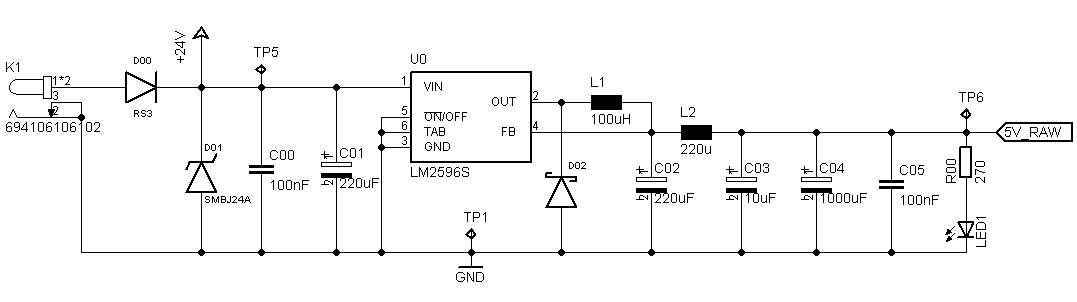
\includegraphics[scale=0.6]{DCDCConverter.png}
			\caption{Circuit diagram of the DC/DC regulator and periferal components}		
			\label{fig:DCDCConverter}
		\end{figure}	
			
		The design incorporates several additional elements:
		
		\textbf{Over voltage protection.} This takes the form of a Transient Voltage Suppressor (TVS) diode anti-parallel with the power source  (D01). Well laid out TVS diodes are designed to have negligible impact on the normal operation of a circuit. The breakdown voltage of the TVS diode is usually in the region of 10\% greater than the reverse standoff voltage which approximates the circuit operating voltage. When a voltage transient occurs that exceeds the breakdown voltage of the TVS diode, it will limit the voltage spike to the TVS diode's clamping voltage and conduct the transient current to ground \cite{VGS_AN88436}.
			
		For this device the SMBJ24A 600\watt\ TVS diode from Fairchild Semiconductor was chosen due to its combined small package size, peak pulse power capability and fast response time. \cite{FS_SMBJ24}

		\begin{wrapfigure}{R}{0.4\textwidth}
			\centering
			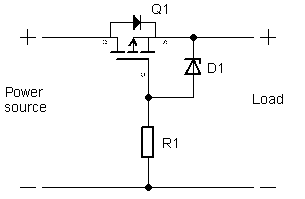
\includegraphics[scale=0.8]{MOSFET_RPP.png}
			\caption{A common protection circuit against reverse polarity}		
			\label{fig:MOSFET_RPP}
		\end{wrapfigure}			
			
		\textbf{Reverse polarity protection.} There are several options for implementing reverse polarity protection. In low voltage systems where a voltage drop can't be afforded, the use of a P-channel MOSFET is common, as its effect on the voltage supply is minimal (Figure \ref{fig:MOSFET_RPP}). 
		
		% more info on this circuit?
		
		For the system being designed a simpler option is acceptable. A rectifier diode is placed in series with the power source (D00). During normal operation the diode is forward biased and current flows to the circuit. Should the polarity of the voltage be reversed, in other words the diode is now reverse biased, the diode will block and the circuit will see no current. The disadvantage of this simpler solution is that the diode exhibits a forward voltage drop; as a result the circuit will no longer receive 24\volt . The rectifier diode chosen for the circuit (see below) has a forward voltage drop of 1.3\volt , so the circuit can expect to see 22.7\volt\ instead of 24\volt . While the nominal operating voltage of the valve is at 24\volt , the operating voltage range lies between 18\volt\ and 30 \volt . Similarly the Measurement amplifier has a nominal supply voltage range of 12\volt\ to 24\volt . In both cases the voltage drop caused by the rectifier is of no consequence.
		
		The RS3G Fast Switching Rectifier from Vishay was chosen for its small package size, high forward current (3\ampere ) and fast switching time.
		
		\textbf{Additional filtering.} In addition to the 220\micro\farad\ input capacitor (C01) stipulated by the DC/DC regulator data sheet, a 100\nano\farad capacitor (C00) was added in parallel to remove high frequency noise. similarly output ripple and noise were further stabilised with an additional 220\micro\henry\ inductor (L2), 10\micro\farad , 1000\micro\farad , and 100\nano\farad capacitors (C03, C04 and C05 respectively). 
		
		% was this tested? yes, not ripple could be detected
		
		\textbf{An indicator LED.} A simple visual indicator placed at the point at which the 5\volt\ produced by the DC/DC regulator enters the BeagleBone Black. The BeagleBone Black should enter its boot procedure once 5\volt\ are connected, so if the LED is on and the boot process doesn't occur, a problem can be inferred.
		
		\subsubsection{Analogue and Digital Power Rails and Ground Planes}
		Digital circuitry is noisy, with rapid switching resulting in current transients and electromagnetic interference in the power supply. The logic levels of digital circuits are themselves virtually immune to these effects, however analogue circuitry powered by the same supply can be vulnerable to induced noise. This is particularly important in signal conditioning circuitry where the fidelity of the signal to be measured is important. Similarly, measurements made with respect to ground need a solid ground. Ground planes underneath digital circuits will suffer from switching noise generated by the digital circuit.   
		
		To minimise the effect of the digital circuitry on the analogue circuitry a separate analogue ground plane and analogue 5\volt\ power rail were introduced. Figure \ref{fig:AnaGND} shows how the regulated 5\volt\ output from the BeagleBone Black was uncoupled from the 5\volt\ analogue power rail. This was achieved with an EMI suppression ferrite bead (L3) and two capacitors (10\micro\farad\ and 100\nano\farad ). Ferrite beads are passive devices that filter high frequency noise by increasing reactance in a specific frequency range and dissipating energy  in the form of heat \cite{AD_AN1368}. The chosen ferrite bead has a maximum impedance at 150\mega\hertz . The ferrite bead is complimented by two capacitors to ground, forming a low pass filter which further suppresses higher frequencies on the supply rail. Space was made for an additional decoupling capacitor (C09) if further filtering is deemed necessary once the board is taken into operation.  
		
		\begin{figure}[H]
			\centering
			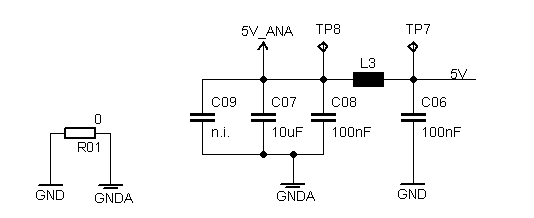
\includegraphics[scale=1]{AnaGND.png}
			\caption{Circuit diagram of the interfaces between the analogue and ground planes (left), and the analogue and digital 5\volt power rails (right)}		
			\label{fig:AnaGND}
		\end{figure}

The circuit of the connection between the digital and analogue ground (Figure \ref{fig:AnaGND}) is simply a 0\ohm\ resistor. In itself, this means nothing, as the resistor has no effect other than to connect the two grounds. However, in practical terms during PCB layout, this enforces the connection of the two ground planes at a single point. Known as star point grounding, the principle of connecting grounds at a single point ensures that all voltages are measured with respect to a particular point, and not just at an undefined "ground" \cite{LinearCircuit}. In many cases a convenient point at which to connect the ground planes is at the power supply. Figure \ref{fig:GNDPlanes} shows the bottom of the developed PCB, with digital ground occupying most of the board. Analogue ground is in the bottom left quarter of the board. The two grounds are completely separate, except for the 0\ohm\ resistor which lies at the top of the board, analogue ground trace that runs up the left hand side of the board. The resistor sits next to the power source and defines the common, defined ground between the two sides of the circuit.

		\begin{figure}[H]
			\centering
			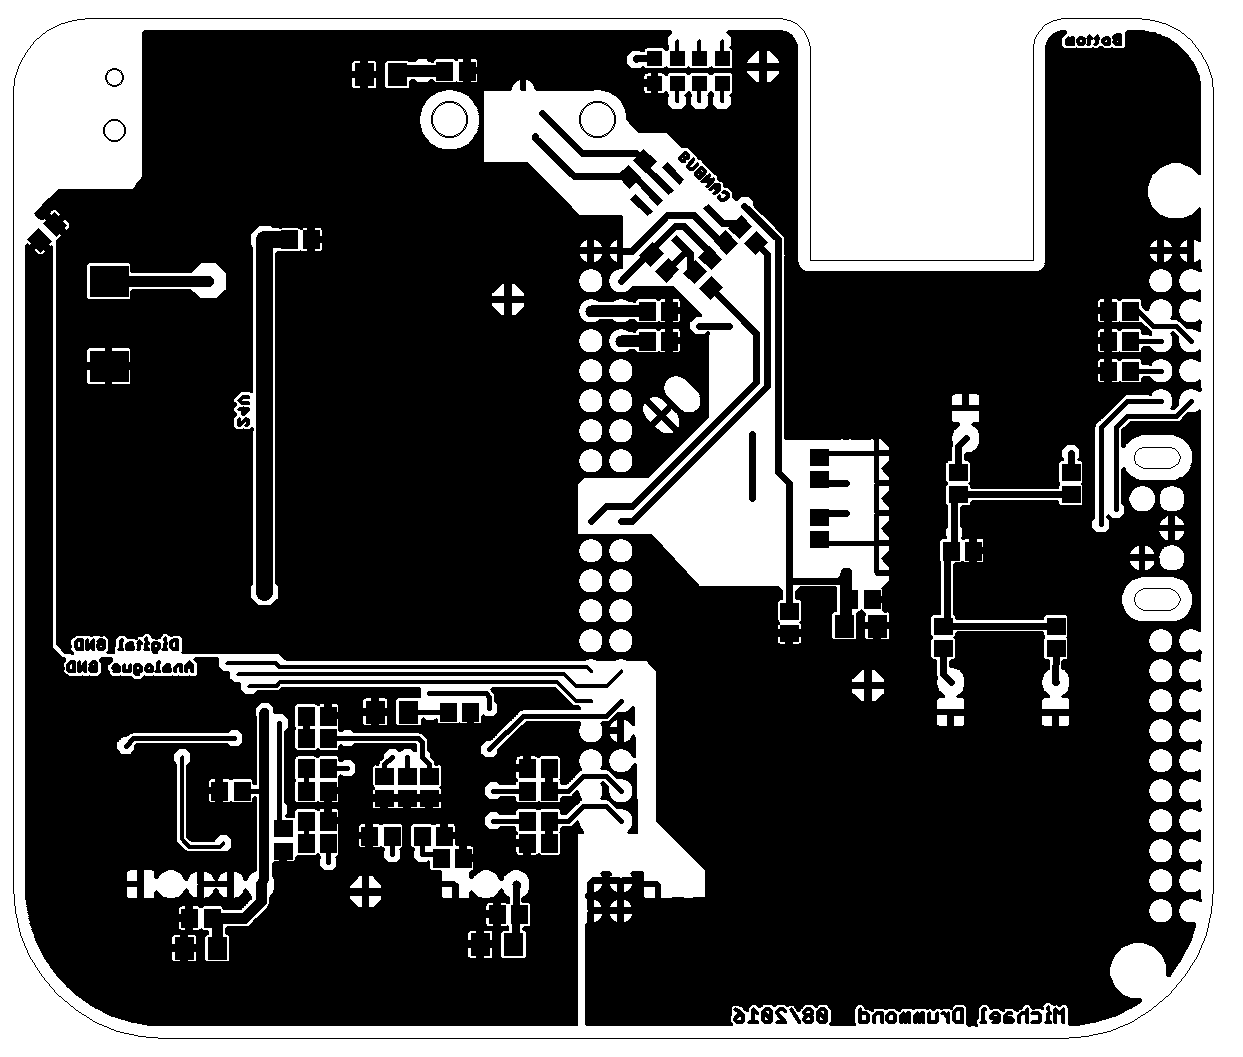
\includegraphics[scale=0.3]{GNDPlanes_negative.png}
			\caption{PCB layout showing the ground planes on the bottom of the board}		
			\label{fig:GNDPlanes}
		\end{figure}

	\subsection{Rotary Encoder and Buttons} \label{sec:Rotary Encoder and Buttons}
		\subsubsection{The Rotary Encoder}	\label{sec:encoder}
		Control and navigation through the device options (see \ref{sec:Menu}) is enabled with the use of a rotary encoder. An encoder or jog wheel was considered a more intuitive interface for setting the valve than a series of buttons, and had the added benefit of giving the device a cleaner appearance. 
		
		The Texas Instruments Sitara processor on the BeagleBone Black includes an Enhanced Quadrature Encoder Pulse (eQEP) Module as part of its Pulse-Width Modulation Subsystem (PWMSS). The eQEP simplifies the implementation of an encoder by decoding its input and making it available to the programmer as a single integer value that is increment or decrement accordingly. In terms of hardware, the two encoder signal lines simply need to be connected to the correct two pins on the BeagleBone Black, and ground to ground. 
		
		The LCD display on the top face of the device and the device's overall compact size meant placing the encoder next to the display was no longer possible. To make its use ergonomic the rotary encoder was moved to the right hand side of the device, and is thus angled at 90\degree\ to the PCB. 
					
		\subsubsection{The Buttons}
		The rotary encoder has a built-in push button switch. This momentary switch allows for the selection of options during the navigation of the GUI. As the device was to include the option of expanding its initial functionality, space for a further three switches was made by including two pin Molex connectors. The switch and the three headers are connected between ground and an individual GPIO pin of the BeagleBone Black, and each include debounce circuitry. 
		
		This takes the form of a low pass filter () followed by a Schmitt trigger...	
		
		\begin{figure}[H]
			\centering
			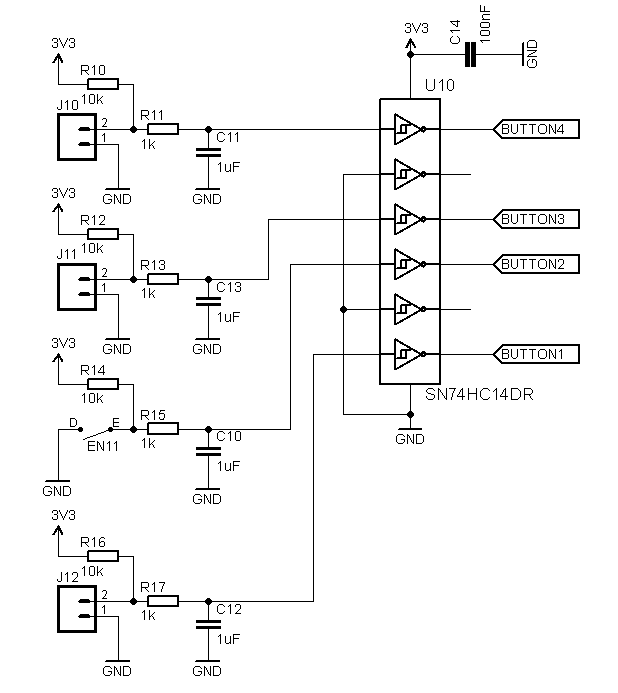
\includegraphics[scale=0.8]{Buttons.png}
			\caption{Debounce circuitry of the buttons. Note the encoder connected to button 2.}		
			\label{fig:Buttons}
		\end{figure}	
		
	\subsection{LEDs}
	In addition to the power supply LED (see \ref{sec:DC/DCRegulator}) a further three LEDs were added to the device to provide someone programming the device with a simple debugging tool or a user with a visual cue that the system is working.
	
	% more info on why they are connected to 5V, why the transistors (current protection of the BBB), those 100kOhm resistors, and maybe current flow through the LEDs and which were chosen
	
		\begin{figure}[H]
			\centering
			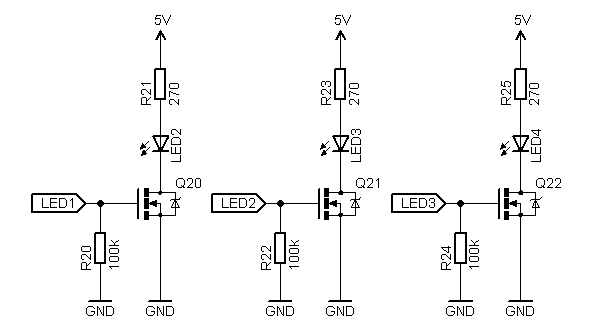
\includegraphics[scale=1]{LEDs.png}
			\caption{The connected LEDs}		
			\label{fig:LEDs}
		\end{figure}	
	
	
	\subsection{Liquid Crystal Display} \label{sec: Liquid Crystal Display}
	The liquid crystal display (LCD) of the device is a 4 line, 20 character, blue backlit display. The LCD's Hitachi HD44780 controller is connected on-board with an I\textsuperscript{2}C interface, cutting down the number of pins required to control the display significantly (from 12 pins in four-bit HD44780 operation, to four pins for I\textsuperscript{2}C). Supply and logic level voltage of the display are 5\volt .	
		
		\subsubsection{I\textsuperscript{2}C} 	\label{sec:I2C}
		
		\subsubsection{Level Shifter}
		Logic level voltage of the BeagleBone Black pins is 3.3\volt, so a bi-directional level shifter circuit was placed between the I\textsuperscript{2}C data (SDA) and clock (SCL) pins and those of the display (Figure \ref{fig:I2C}). The level shifter ensures that the 3.3\volt\ logic signals from the BeagleBone Black are read as 5\volt\ signals at the display.
		
		The circuit involves an n-channel MOSFET (Q30 and Q31) placed on each of the signal lines (SDA and SCL), with source connected to the 3.3\volt\ bus line and drain to the 5\volt\ bus line. These are flanked by pull-up resistors to the two power rails (R30 to R33). The gates of both MOSFETS are connected to the lower voltage supply rail (3.3\volt ).
		
		In this configuration, if neither side is pulled down, the pull-up resistors result in 3.3\volt\ at one end of the bus line and 5\volt\ at the other. Should the 3.3\volt\ end of the bus line be pulled down, \volt \textsubscript{GS} will rise, the MOSFET conduct and the 5\volt\ end of the the bus will also be pulled down. Equally, should the 5\volt\ end of the bus be pulled down, the body diode of the MOSFET will conduct, again drawing \volt\textsubscript{GS} down until the MOSFET conducts and the bus line is pulled down to the same level at both ends. \cite{NXP_AN10441}    
		
% need and explanation of R34 and R35
		
		
		\begin{figure}[H]
			\centering
			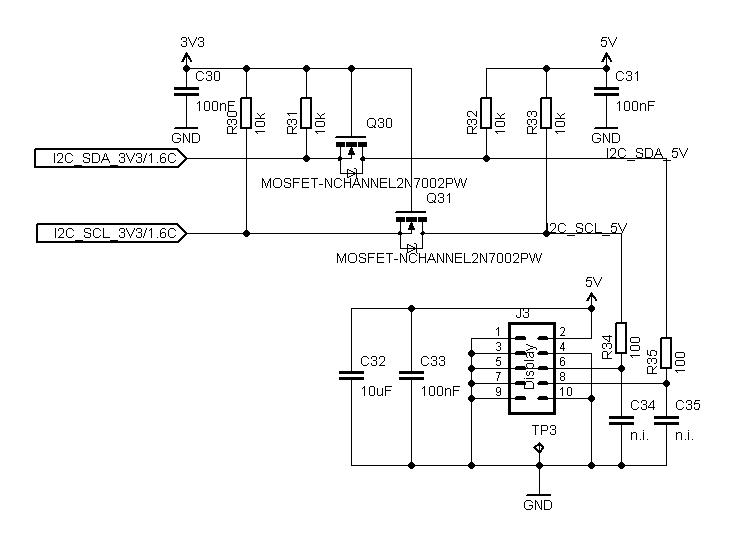
\includegraphics[scale=0.85]{I2C.png}
			\caption{The logic level shifting circuit between the I\textsuperscript{2}C pins of the BeagleBone Black and those of the display}		
			\label{fig:I2C}
		\end{figure}
				
	\subsection{CAN bus} \label{sec:CAN}
	% include an explanation of why we need this. ie to control the valve (actuator), and how that ties in with the control loop
	% Include a broader description of what CAN is. differential signal etc...	
	
	The AM335x processor on the BeagleBone Black incorporates a module for accessing a Controller Area Network (CAN) bus. The DCAN module provides support for CAN protocol version 2.0 at bit rates up to 1MBit/s \cite{TechRefMan}. The AM335x includes two instantiations of the DCAN controller (DCAN0 and DCAN1), both are connected to pins on the P9 header of the Beaglebone Black \cite{BBB_SRM}. Due to the high frequency switching on the RXD and TXD lines of the CAN controller these should not be placed over a ground plane. The RXD and TXD of DCAN1 are connected to pins 24 and 26, but their use would interfere with the ground plane that extends from the left to the right side of the board. The ground plane is itself constrained by the analogue circuitry at the bottom left of the board. For this reason, DCAN0 with its RXD and TXD lines connected to pins 19 and 20 was chosen to provide the CAN controller.	
	
		\subsubsection{CAN Transceiver}
		Additional hardware, in the form of a transceiver, is required for the connection to the physical CAN bus \cite{TI_SLLA270}. As the RXD/TXD pins of the BeagleBone Black operate at 3.3\volt an appropriate 3.3\volt CAN bus transceiver was needed. For this the Texas Instruments SN65HVD232 was chosen (U40, Figure \ref{fig:CANbus}). Following the data sheet layout guidelines, serial resistors (R40 and R41) were placed to limit current on the digital lines \cite{CANbus_transceiver}. An optional pull up resistor (R42) was used to drive the recessive input state of the transceiver. High speed CAN (see ISO 11898-2\cite{ISO11898}) requires termination resistors at both ends of the transmission lines. The resistors match the nominal impedance of the cable, which the CAN standard specifies as 120\ohm . R43 is such a termination resistor, placed as close to the CAN High and CAN Low pins of the transceiver as possible. In addition, a bypass capacitor was placed as close as possible to the supply pins of the transceiver (C40), and bulk and bypass capacitors were placed on the 24\volt\ supply line of the valve (C41 and C42).
		
		\begin{figure}[H]
			\centering
			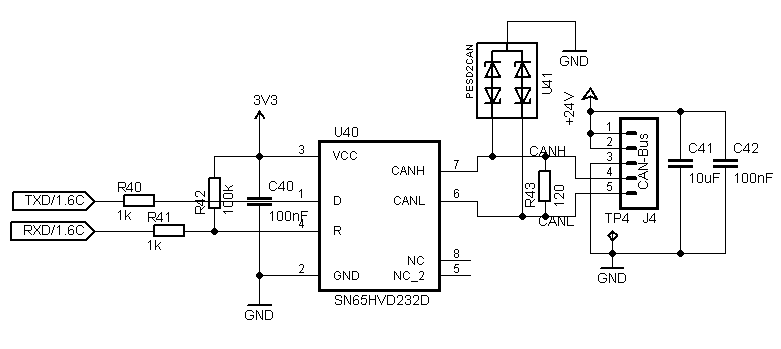
\includegraphics[scale=0.82]{CANbus.png}
			\caption{CAN transceiver, ESD protection diodes, and circuitry connecting the on-board CAN controller with the CAN bus}		
			\label{fig:CANbus}
		\end{figure}		
		
		\subsubsection{CAN Bus Circuit Protection}
		The on-chip electrostatic discharge (ESD) protection of the CAN transceiver is good enough for many applications, but insufficient for electrical fast transients (EFT) and surge transients occurring in industrial environments\cite{CANbus_transceiver}. While this device is unlikely to leave the laboratory, good practice in designing a robust and reliable bus node was followed and additional circuit protection was added. This took the form of a CAN bus ESD protection diode from NXP Semiconductors (PESD2CAN, U41 in Figure \ref{fig:CANbus}). This was placed close to where the bus connects with the board to prevent the transients from propagating on the PCB.  
		
	\subsection{Analogue Inputs} \label{sec:AnalogueInputs}
	The analogue inputs are core elements of the device. Input from the pressure sensor is used in the control function to find the pressure set point selected by the user. The accurate setting of the muscle is conditional on the accuracy of the feedback response measured by the pressure sensor. Once the set point has been reached, the device takes a force measurement from the force sensor. This data underpins the measurement of the static force characteristic of the PMAs, and so its accuracy is likewise essential.
	
	The AM335x processor of the BeagleBone Black includes a subsystem with an 8-channel general-purpose analogue-to-digital converter (ADC), with optional support for interleaving touchscreen conversions for a resistive panel (abbreviated to TSC\_ADC\_SS)\cite{TechRefMan}. 
	
	The subsystem comprises of a single 12 bit Successive Approximation Register (SAR) ADC that is multiplexed to the 8 channels. The ADC will measure voltages between 0 and 1.8\volt. The 1.8\volt\ supply that drives the ADC is provided as a voltage reference on a pin of the BeagleBone Black, as is an analogue ground pin. Both the pressure and force input signals require conditioning to bring them within the voltage span of the ADC. In both cases this was achieved with a simple voltage divider (Figures \ref{fig:Pressure} and \ref{fig:Force}). 
	
	The ADC has a maximum sampling rate of 200\kilo\hertz . This is significantly faster than the sub kilohertz sampling rate anticipated for the device, even if measurements are taken from two channels. The sampling frequency determines the input impedance of this ADC, so with both pressure and force measurements each taken at 100\hertz\ the input impedance equates to \cite{TI_AM335x}
	\begin{align*} 
		\frac{1}{65.97{\times10^{-12}} \cdot 200\hertz } \approx 75.8\mega\ohm
	\end{align*}
	While this input impedance may be sufficient given the device's current application, a change (for example) in measurement frequency could easily bring the introduced error caused by input overloading to an unacceptable level. For this reason a unity-gain buffer was placed between the voltage dividers and the ADC input (Figures \ref{fig:Pressure} and \ref{fig:Force}). This impedance matching was implemented with the MCP6004 quad op-amp IC from Microchip Technology inc.
	
	% this also prevents excessive current draw that could damage the adc input
	
	A further consideration was the small capacitor that the sample and hold element of the ADC uses. This can cause problems for the buffer's op-amp at high sampling frequencies. If the dynamics of the op-amp are too slow, the capacitive load on the op-amp can result in settling times that can skew the result. To deal with this, a simple RC filter can be placed between the buffer output and ADC input. Space for such filters were made in the design, but given the low sampling frequencies planned for this device, they were not instantiated.

		\subsubsection{Voltage Reference} 			\label{sec:ADCVoltage}
		The BeagleBone Black 1.8\volt\ ADC voltage reference pin was used to drive four op-amps required for impedance matching in the signal conditioning circuitry of the analogue inputs (described above). To prevent the circuit drawing a current that could damage the BeagleBone Black, the output of the voltage reference pin was itself buffered, as in Figure \ref{fig:VREF}. The component used here was a MCP6001 single op-amp, supplied by the 5\volt\ analogue rail. In addition to a 100\nano\farad\ bypass capacitor, a 10\micro\farad\ bulk capacitor and 5\ohm\ resistor were placed at the end of the 5\volt\ supply to prevent any drops in the supply and maintain an accurate reference.
		
		\begin{figure}[H]
			\centering
			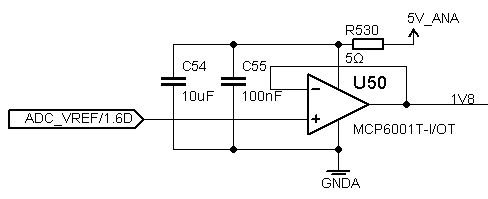
\includegraphics[scale=0.85]{VREF.png}
			\caption{VREF}		
			\label{fig:VREF}
		\end{figure}				
		
		\subsubsection{Pressure Sensor}
		The 1.8\volt\ voltage reference supplies the quad op-amp IC, of which one op-amp is used in the signal conditioning of the pressure sensor input (Figure \ref{fig:Pressure}). The pressure sensor is supplied by the analogue 5\volt\ rail, filtered and supported by bypass and bulk capacitors. The sensor output is a value between 0 and 5\volt\ which is paired down in a voltage divider to bring it to between 0 and 1.8\volt . Resistors with  0.1\% tolerance were selected to improve accuracy. The voltage divider is followed by a unity gain buffer to match the divider's impedance to that of the analogue input pin of the BeagleBone Black (described above). The total resistance of the divider was aimed in the region of 150\kilo\ohm . The relatively high resistance prevents the sensor measurement from being negatively impacted by a high current draw. Moreover, the unity gain buffer negates the problems the high resistance of the divider might cause with the ADC input. 
		
		The pressure sensor was connected with AIN0 of the BeagleBone Black.
		
		\begin{figure}[H]
			\centering
			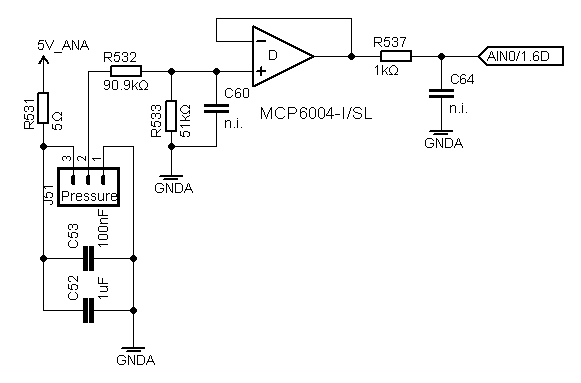
\includegraphics[scale=0.85]{Pressure.png}
			\caption{Pressure}		
			\label{fig:Pressure}
		\end{figure}		
		
		\subsubsection{Force Sensor}
%what type of force sensor is it actually? and mention to measurement applifier too 		
		
		The signal conditioning circuitry connecting the force sensor to the BeagleBone Black is built on a similar set-up to that of the pressure sensor. That is to say, a voltage divider pairs the signal down to between 0 and 1.8\volt\ and a unity gain buffer matches the impedance to that of the input of the ADC. However, several further additions enhance the accuracy of the measurements (Figure \ref{fig:Force}).		
		 
		The PMAs to be tested by the rig are available in different diameters, from 5\milli\meter\ to 40\milli\meter . The larger the diameter of the PMA, the greater the force that it is able to exert. So, while the force sensor and external measurement amplifier are set up to read a force up to ??\newton\ and convert it to a voltage between 0 and 10\volt , the maximum voltage output will only ever be reached by the very largest muscles. It is, therefore, only the force measurements of these PMAs that will use the full span of the 12 bit ADC on the BeagleBone Black, and that of the smaller PMAs will have a corresponding loss in resolution. To compensate for this, three voltage dividers with differing ratios were implemented. A CMOS analogue switch (U52, a Maxim MAX4662) placed before the dividers allows the user of the device to choose between them. During use only one switch will be "on" at any given time, and the signal will pass through this divider to be read by one of the ADC channels. 
		
		%something about the choice of analogue switch
		% what pins are the switches connected to
		%possible discussion on where and how the switch could have been set up (before/after each stage)
		
		The voltage dividers themselves are composed of 0.1\% tolerance metal film resistors. To improve accuracy and their flexibility in use, each divider is made up of two pairs of resistors in series. In so doing, sourcing appropriate resistor values for the divider ratio was made easier. The voltage divider ratios, and the switches they are connected to, are listed in table \ref{tab:VoltageDividers}. The user will select the input path based on the maximum voltages expected. For any given signal input path the dividers will convert the signal from between 0\volt\ and the respective maximum input voltage to between 0 and 1.8\volt .
		
		\begin{table}[H]
			\centering
			\footnotesize
			\renewcommand{\arraystretch}{1.5}
			\begin{tabular}{p{5cm} c c}
			& \multicolumn{2}{c}{\textbf{Voltage divider}} 
				\\ \cline{2-3}
				\textbf{Analogue switch} 	& \textbf{Max. input} [\volt] 	& \textbf{Ratio}
				\\ \hline 
				Switch 1					& 3.3							& 1.8$\overline{\mbox{33}}$ 
				\\ \hline 
				Switch 2					& 10 							& 5.55
				\\ \hline 
				Switch 3					& 6								& 3.34 
				\\ \hline
			\end{tabular}
			\renewcommand{\arraystretch}{1}
			\caption{Analogue force sensor voltage dividers. Output voltage of the dividers is in all cases between 0 and 1.8\volt given an input between 0\volt\ and the maximum input of the signal path chosen by the switch.}
			\label{tab:VoltageDividers}
		\end{table}	
		
		\begin{sidewaysfigure}
			\centering
			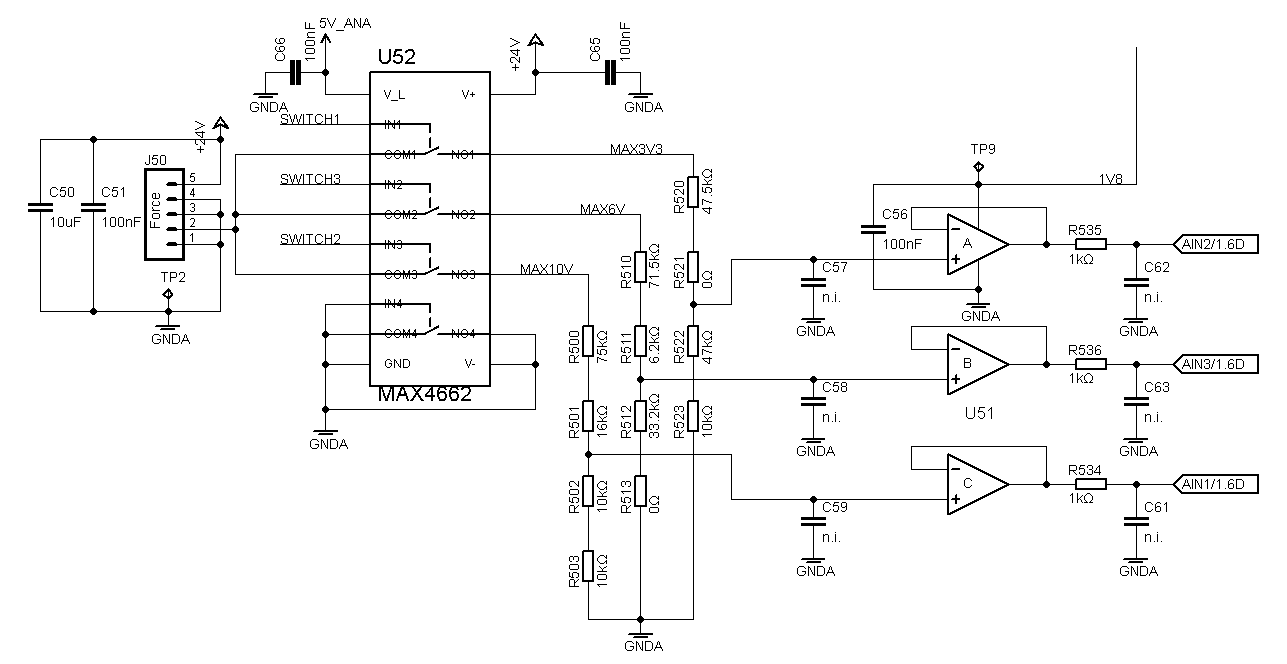
\includegraphics[scale=0.75]{Force.png}
			\caption{Force}		
			\label{fig:Force}
		\end{sidewaysfigure}			
		
\section{Software Development}
	\subsection{Outline}
	The BeagleBone Black can run a fully fledged Linux operating system, courtesy of the Texas Instruments AM3358 ARM Cortex-A8 processor. Debian 8.6 (Jessie) was installed on the device, and a remote debugging environment was set up according to the instructions in chapter 7 of \cite{ExploringBeagleBone}. 
	
	The development of the software can conceptually be divided into five areas. The first three form the core of the device's function: 

	\begin{itemize}
	\item The analogue to digital conversion of the pressure and force inputs
	\item The CAN bus output to the compressed air valve
	\item The PID controller links the pressure sensor with the valve actuator
%why PID?	
	\item Storage of the recorded data on removable media
	\item The user interface. Fundamental to the user's interaction with the device. Primarily this is the menu, but also includes the initialisation and communication between the BeagleBone Black and the display and encoder.
	\end{itemize}		
	 
	 A standard Linux kernel, such as the one that Debian is built on, is a preemptive kernel. Preemptive scheduling has many advantages, but it cannot execute tasks in real time. This is problematic in implementations of discrete-time PID controllers that are called upon to act at specific time intervals. 
	 
	 The BeagleBone Black's AM3358 includes a Programmable Real-Time Unit Subsystem and Industrial Communication Subsystem (PRU-ICSS), which provides a convenient way to implement real-time functionality where it is needed. The PRU-ICSS can be thought of as two 32 bit on-chip microcontrollers running at 200\mega\hertz (known as PRUs). They have full access to the internal memory of the processor and it's peripherals, and single-cycle IO access to a number of pins (but not all). So, for example, an initial mock-up of the test rig had a PRU reading pressure values from the ADC and outputting a Pulse Width Modulation (PWM) signal to a valve. The PRU has single-cycle access to the ADC values, and the software defined PWM output used a GPIO pin.
	 
	 The PID controller would have been implemented with the help of an on board single-cycle 32 bit multiplier, however, external factors led to the PWM valve being replaced with a CAN-bus valve. The PRUs don't have direct access to the DCAN module that performs CAN protocol communication on the AM3358, so a hard real-time set-up of the control system fully implemented using the Programmable Real-Time units was no longer possible.
	 
	 To keep the control system simple, yet keep some of the benefits of the PRU-ICSS, the control system was programmed in Linux space, while an accurate timer was implemented using one of the PRUs. The PRU generates an interrupt at precise time intervals, that alert the controller running in a high priority thread in Linux space to calculate a new output value. 
	 
	 
	 % a service is called to start the program after system boot
	 
	\subsection{Device Tree Overlays}
	The device tree is a data structure for describing hardware, that obviates the need to hard code details of a device into an operating system. Aspects of the hardware can be described in the device tree, which is passed to the operating system at boot time. Device Trees have become mandatory for all new ARM SoCs, and Debian Jessie (used on this device) is built on the Linux kernel version 3.16, which implements the Flattened Device Tree (FTD) model \cite{DeviceTree}. To enable runtime configuration of inputs and outputs on the BeagleBone Black, a system of Device Tree Overlays (DTOs) and a cape manager exist \cite{capemgr}.

	The following device tree .dts files were programmed, compiled as device tree binary overlays (.dtbo), and place in the /lib/firware folder. At boot, the system loads the .dtbo files to extend the device tree.
	
	% parts of the following needs to be moved to the hardware section
	
	\begin{itemize}
		\item \textbf{ADC.dts} Enables the use of the ADC channels 0 to 6. Pins 32 to 40 of the P9 header are exclusively used by the ADC. These pins include the voltage reference and analogue ground (described in \ref{sec:AnalogueInputs}) along with the 7 aforementioned input channels.
		\item \textbf{DCAN0.dts} Enables one of the DCAN controller modules that performs CAN protocol communication on the AM3358. DCAN0 was enabled for PCB design layout considerations (see \ref{sec:CAN}). RXD and TXD of DCAN0 are multiplexed to pins 19 and 20 of the P9 header of the BeagleBone Black. As the I\textsuperscript{2}C2 bus is set to default on these pins,  it was first necessary to modify the device tree binary that is used at boot (am335x-boneblack.dtb). This involved decompiling the binary, commenting out the section related to I\textsuperscript{2}C2 (starting line 78), recompiling and rebooting.
		\item \textbf{eQEP2.dts} The Enhanced Quadrature Encoder Pulse (eQEP) Module (described in \ref{sec:encoder} of the AM3358 chip provides an easy way to implement a quadrature encoder. Two of these modules are provided for on the BeagleBone Black; both on the P8 header. The rotary encoder was placed on the right-hand side of the device necessitating the removal of pins 13 to 26 of the P8 header. While both eQEP modules were still accessible, the placement of the buttons and their connection to pins 27 to 30, meant connecting the encoder to eQEP2 was the parsimonious choice. 
		
		%was this mentioned in the hardware section?! about the removal of pins for the encoder?
		
		\item \textbf{GPIOs.dts} Enables the pins 7 to 9 on the P8 header as outputs for the LEDs. In addition, pins 27 to 30, also on the P8 header, are configured as inputs. All seven pins are pulled down with no signal. 
		\item \textbf{I2C1.dts} With I\textsuperscript{2}C2 disabled to allow for DCAN0, and I\textsuperscript{2}C0 not exposed on the expansion headers, only I\textsuperscript{2}C1 was available to communicate with the display. The data (SDA) and clock (SCL) lines of the I\textsuperscript{2}C1 module are available either at pins 17 and 18 or pins 24 and 26 of the P9 header. To maximise space for the ground plane (see \ref{}) the module was connected to pins 24 and 26.
		\item \textbf{PRU.dts} The Programmable Real-Time Units are also enabled over a device tree overlay. In this case both PRUs were enabled, although only one is used. Furthermore, a debug pin (pin 27 on header P9) was enabled to help verify the timer instantiated on the PRU.
	\end{itemize}
	
	%mention the removal of mcasp0 (see notes) to allow for the placement of the switch pins
	
	
	\subsection{User Interface} \label{sec: User Interface}
	The user interacts with the device through an options menu with the help of a rotary encoder and display (described in \ref{sec:Rotary Encoder and Buttons} and  \ref{sec: Liquid Crystal Display}).
		\subsubsection{I\textsuperscript{2}C and LCD}	
		Header and source files (lcdDisplay.h and lcdDisplay.cpp) were developed to take care of the I\textsuperscript{2}C interface to the display and the commands for the LCD itself. The contents of the files is heavily based on a python library for Raspberry Pis with similar functionality \cite{LCD}. Additional functions that were added, improve the programmer's options in terms of which types can be placed on the display (eg int and float), and the position at which they can be displayed (left or right-hand side).	
		
		% http://blog.chrysocome.net/2013/03/programming-i2c.html      for initI2C()		
		% http://hardware-libre.fr/2014/03/en-raspberry-pi-using-a-4x20-characters-display/     for everything else
		
		Following the boot process and the launch of the underlying device software, two things happen related to the display. First, access to the I\textsuperscript{2}C bus is opened and communication with the slave LCD device is initiated with its I\textsuperscript{2}C address. This occurs with the initI2C() function. Second, the initLCD() function initialises the LCD, a display that uses the Hitachi HD44780 protocol, in 4-bit interface mode \cite{HD44780} (Listing \ref{lst:I2C}). At this stage the LCD is initialised and ready to display the menu or messages to the user.
		
		\lstinputlisting[	firstline = 167, 
	                 		lastline = 169, 
	                 		firstnumber = 167,
	                 		label= lst:I2C,
	                 		caption = Accessing the I\textsuperscript{2}C bus and initialising the display]
							{/home/mkadrummond/workspace/Beaglebone/src/main.cpp} 	
		
		\subsubsection{Rotary Encoder and Button}
		The C++ eQEP API written by Nathaniel Lewis \cite{eQEP_API}	was used as the interface to the eQEP driver. The main function creates an instance of the eQEP class based on the root path of the eQEP2 sysfs entry, and the operating mode of the hardware. In this case the eQEP hardware is run in absolute mode (Listing \ref{lst:encoder}). This means its position starts at zero and is incremented or decremented by the encoder's movement, as opposed to being reset after a time interval. 	
		
		Following instantiation, the period at which the eQEP hardware polls the input is set with the set\_period() function. Smooth operation of the encoder with the menu was achieved with a period of 10\milli\second (or 10,000,000\nano\second ).
		
		\lstinputlisting[	firstline = 173, 
	                 		lastline = 175, 
	                 		firstnumber = 173,
	                 		label= lst:encoder,
	                 		caption = Setting up the encoder]
							{/home/mkadrummond/workspace/Beaglebone/src/main.cpp} 
							
		% button!
		
		\subsubsection{Menu}						\label{sec:Menu}
		A menu was created to allow a user of the device to select and change parameters of the test rig. The underlying structure entails a class of menu nodes (class MenuNode, described in menu.h and menu.cpp), in which instantiated MenuNode objects contain a vector of further MenuNodes (simply named \textit{v}). Each MenuNode has a useNode() function that is defined with a function pointer at object instantiation. In this way, the user can pass the MenuNode a function defining  what should happen when the node is "used". 
		
		Conceptually one can differentiate between internal and terminal nodes, although this distinction isn't made in the software. Internal nodes will, when their useNode() function is called, display the contents of their MenuNode vectors, allowing the user to navigate further into the menu. In contrast, terminal nodes will display settings that can be changed by the user.

		Besides a \textit{name} variable and the aforementioned vector, MenuNode objects contain the member variables vectorCursor and displayOffset. The first, is essentially an iterator for the vector. When linked with the encoder input, this variable allows the user to navigate the vector, and by extension, the menu. The displayOffset variable is needed for displays that have fewer lines than the length of any given MenuNode vector. In these cases, the lines that are displayed need to change depending on the vectorCursor position in the vector.

		The display and navigation of MenuNode vectors is facilitated with the two functions displayMenu() and updateDisplay() (at the end of main.cpp). These functions use the member variables vectorCusrsor and diplayOffset to display the appropriate nodes of the MenuNode vector and cursor position on the LCD.  		
		
		
				
		
	\subsection{Control System}	
		\subsubsection{Analogue to Digital Conversion}
		% a word on the sampling frequency. These are dc signals, so sampling freq is not critical in that sense. However, the pressure measurement freq is critical to the control function 	
	
		\subsubsection{CAN bus}
		\subsubsection{PID Controller with PRU Timer}
	\subsection{Data Storage}
\section{Data Acquisition}
\section{Discussion}
\section{Conclusion}

\newpage

%\bibliographystyle{plain}
%\bibliography{/Users/mkadrummond/Documents/Elektrotechnik/Bachelorarbeit/Thesis/Bibtex/library}{}


\begin{thebibliography}{1}
\bibitem{BBB_SRM}
	G. Coley, \textit{BeagleBone Black System Reference Manual, Revision C.1}, May. 2014
	
\bibitem{TI_LM2596}	
  Texas Instruments, \textit{LM2596 Simple Switcher \textsuperscript{\textregistered} Power Converter 150kHz 3A Step-Down Voltage Regulator}, 2013	
  
\bibitem{VGS_AN88436}	
  Vishay General Semiconductor, Appl. Note 88436, \textit{What is a Silicon Transient Voltage Suppressor and how does it work?}, 2007
	
\bibitem{AD_AN1368}	
  Analog Devices, Appl. Note 1368, \textit{Ferrite Bead Demystified}, 2015
  
\bibitem{FS_SMBJ24}	
  Fairchild Semiconductor,  \textit{SMBJ5V0(C)A - SMBJ170(C)A 600 Watt Transient Voltage Suppresssors}, SMBJ24A datasheet, 2003 
  
\bibitem{NXP_AN10441}	
  NXP Semiconductors, Appl. Note 10441, \textit{Level shifting techniques in I\textsuperscript{2}C-bus design}, 2007
  
\bibitem{LinearCircuit}	
  H. Zumbahlen, \textit{Linear Circuit Design Handbook}. Amsterdam, Netherlands: Elsevier Ltd, 2008
  
\bibitem{TechRefMan}	
  Texas Instruments Technical Staff, \textit{AM335x ARM\textsuperscript{\textregistered} Cortex\texttrademark -A8 Microprocessors (MPUs) Technical Reference Manual}. Texas Instruments, Oct. 2011 [Revised Apr. 2013]
  
\bibitem{TI_SLLA270}	
  Texas Instruments, Appl. Note SLLA270, \textit{Controller Area Network Physical Layer Requirements}, Jan. 2008

\bibitem{CANbus_transceiver}	
  Texas Instruments, \textit{SN65HVD23x 3.3-V CAN Bus Transceivers}, Mar. 2001 [Revised Jul. 2015] 	
  
\bibitem{ISO11898}	
  \textit{Road vehicles -- Controller area network (CAN) -- Part 2: High-speed medium access unit}, ISO 11898-2:2003
  
\bibitem{TI_AM335x}	
  Texas Instruments,  \textit{AM335x Sitara\texttrademark Processors}, AM335x datasheet, Oct. 2011 [Revised Apr. 2016]
  
\bibitem{ExploringBeagleBone}
  D. Molloy, \textit{Exploring BeagleBone: Tools and Techniques for Building with Embedded Linux}, 2015
  
\bibitem{DeviceTree}
  devicetree.org, "The Device Tree Specification," 2016 [Online]. Available: http://www.devicetree.org [Accessed: Nov. 07, 2016].   
  
\bibitem{capemgr}
  eLinux.org, "Capemgr," Sep. 20, 2015 [Online]. Available: http://www.elinux.org/Capemgr [Accessed: Nov. 07, 2016]

\bibitem{LCD}
	Captain Stouf, "Raspberry Pi: using a 4x20 characters display," Mar. 20, 2014 [Online]. Available: http://hardware-libre.fr/2014/03/en-raspberry-pi-using-a-4x20-characters-display [Accessed: Mar. 24, 2016]
	
\bibitem{HD44780}	
  Hitachi,  \textit{HD44780U (LCD-II), Dot Matrix Liquid Crystal Display Controller/Driver}, HD44780U datasheet, Sep. 1999
   
\bibitem{eQEP_API}
  Nathaniel Lewis, "C++ eQEP API," May. 15, 2014 [Online]. Available: https://github.com/Teknoman117/beaglebot/tree/master/encoders/api/c\%2B\%2B [Accessed: Apr. 21, 2016]


\end{thebibliography}

\end{document}